% !TEX spellcheck = uk_en
\documentclass[main.tex]{subfiles} 

\begin{document}

\section*{Undervisningsopplegget}
\label{sec:1}

% \subsection*{Microsoft OneNote}

% I undervisningen ble OneNote brukt til de første to timene. OneNote er en dataprogram som lar 
% brukere inntaste enten fra tastatur, eller kan anvendes sammen med en smartboard med en stylus til å
% føre håndskrevne notater. Bilder, tabeller og videor kan settes inn i notatene. Sidene i notatene 
% blir lagret automatisk og organisert i seksjoner i notatboken. Isteden for tavleundervisning, 
% ble OneNote brukt til å føre forelesningsnotater, og i et av sekvensene ble 
% digitalerepresentasjoner brukt til å fremstille organsystemer (se figurene \ref{fig:notat1} -
% \ref{fig:notat2}). Disse notatene blir lagret på nettskyen, som elevene kan ha lesetilgang til
% fra sine private koblinger. Elevene har ikke tilgang til egne maskiner i timene (siden dette 
% strider mot skolens ordensregler om bruk av mobiler og andre verktøy i timen), med mindre en 
% så-kalt laptoptralle blir hentet til klassen av underviseren. En slik tralle inneholder flere 
% pcer som elevene låner midlertidig for å utføre skolearbeid. I våre timer valgte vi å ikke 
% benytte laptoptrallen siden undervisningen ble ført på lystavlen og elevene ble isteden bedt 
% om å ta skriftlige notater. Noe som viser seg ikke er normen, med mindre elevene blir 
% eksplisitt bedt om å ta notater. Dette vil jeg senere gå nærmere inn på når jeg analyserer 
% undervisningssekvensene.

\begin{figure}[h!]
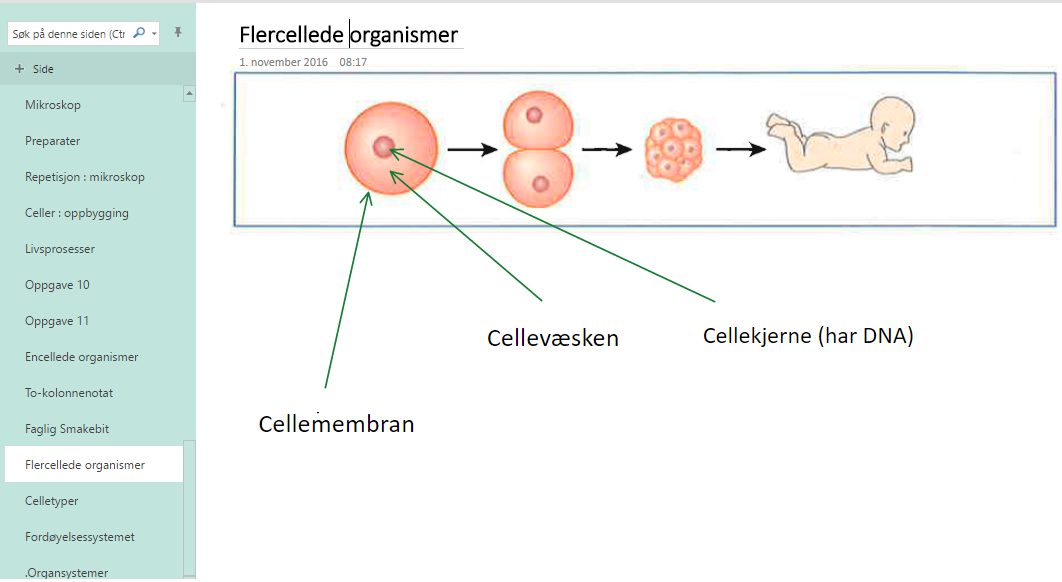
\includegraphics[scale = 0.6]{../figures/onenote_flercellet.png}
\caption{notat 1}
\label{fig:notat1}
\end{figure}

\begin{figure}[h!]
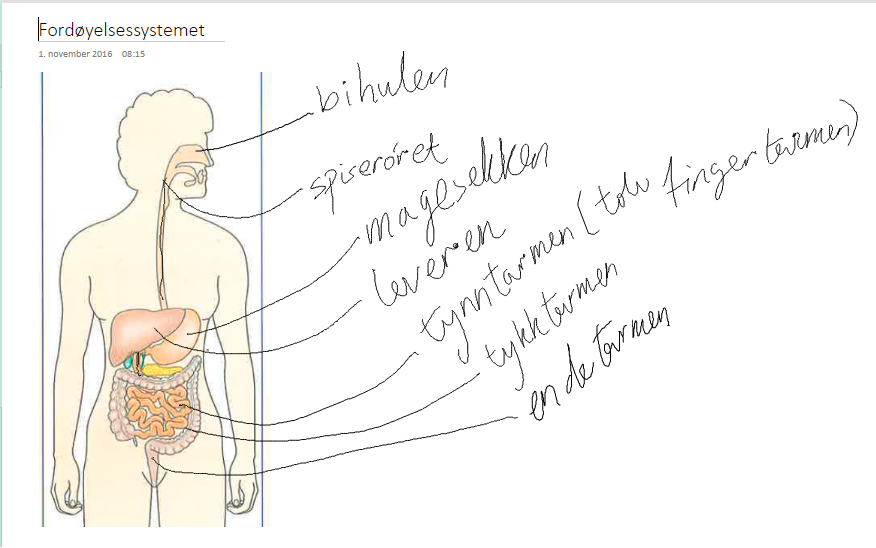
\includegraphics[scale = 0.6]{../figures/onenote_fordoyelse.png}
\caption{notat 2}
\label{fig:notat2}
\end{figure}

\subsection*{1. time}
Undervisningen er fordelt på 3 skoletimer over 2 uker. Opplegget utførte jeg alene, 
med veileder og en medstudent som observatører. De bidro også i blant med å gi veiledning når elevene jobbet
enten selvstendig eller sammen i grupper.

Hensikten med denne timen er å oppsummere det elevene har lært hittil om celler og 
levende organismer, og innføre et nytt tema om encellede organismer. Timen starter med repetisjon 
av det elevene har lært fra tidligere timer, deriblant om mikroskop og cellestrukturen. Ved oppstart 
av timen initieres elevene til å reflektere over temaer og begreper de har lært og hatt lekser 
om. IRE/F metoden <legg til forklaring> brukes, der elevene som rekker opp hånda blir spurt. Det viser seg at det 
er noen få elever, som viser trygghet og kontroll når de responderer til lærer initiert dialog. 

% En av de viktigste egenskapene en lærer kan utvise er evnen til å tilpasse seg i forhold til 
% klassen, en gruppe eller på individ nivå. Ved å erkjenne at alle elevene skal ha kjennskap til 
% begrepene som blir tatt opp og repetert, er det da nødvendig å få bekreftet at elevene innehar en 
% overordnet forståelse. Det kan derfor være nødvendig å frempeke noen elever som ikke viser aktiv 
% deltagelse i timen og frembringe deres respons. Derimot er dette problematisk hvis det viser seg at 
% de ikke har forutsetninger til å kunne respondere. Da settes de i en vanskelig situasjon hvor det 
% blir nødvendig for læreren å lede de ut, ved hjelp av for eksempel ledende spørsmål. Derimot hvis 
% det er forventet at det er en del av forutsetningene at elevene skal kunne respondere til lærer 
% initiativ, da kan utspørringen av elevene vise hull i deres kunnskap. I neste time blir en 
% annen form for lærer initiativ brukt til å frembringe respons. 
 
Siden elevene gjennom helklassesamtalen har blitt "varmet" opp kognitivt, er de mottagelige for å 
lære om et nytt tema. Innføringen av nytt tema er bevisst satt opp på en slik måte at overgangen 
fra repetisjon til det nye temaet blir naturlig og flytende. Dette vil bidra til å la elevene danne et 
helhetlig bilde om celler. I timene hvor de har hatt en innføring om celler, har de lært om basale 
strukturer. I denne timen går de litt dypere ved å få en innføring om en av klassifikasjonene av celler.
Hensikten med innføringen er todelt : å gjøre elevene bevisst om at det finnes forskjellige type
celler, og gjøre de klar for den siste timen hvor de vil studere slike celler under mikroskop.

%Siden det er til hensikt å bruke resterende del av timen til repetisjon, er det ikke nødvendig å 
%prøve å finne svakheter i elevenes respons gjennom helklassesamtalen. For å finne slike svakheter 
%ble gruppesamtalene en bedre plattform. I den forbindelse ble tokolonnenotatet tatt i bruk (se 
%vedlegg : \ref{sec:tokolonnenotat}). 
I den siste øvelsen skal elevene jobbe sammen med tokolonnenotatet (se 
vedlegg : \ref{sec:tokolonnenotat}) i grupper, hvor de blir enige med hverandre om hva som er viktig å 
være formidle videre om deres felles temaer. 
Deretter fordeles de i nye grupper slik at hver gruppe har minst en elev som har forbredt sitt sett 
med temaer/begreper. Under hele denne prosessen er vi tilgjengelige og går rundt for å høre elevene 
diskutere begreper, først sammen i grupper, og deretter individuelt når de fremfører sine 
konklusjoner med medelever. Hvis vi observerer at eleven har problemer med å gi tilstrekkelig 
respons på et gitt tema, initierer vi eleven i en dialog hvor vi forsøker å sammen konstruere en 
mer utdypet forståelse av begrepene, og vi lar andre elever i gruppen være med på dialogen. 

\subsection*{2. time}

% Timen starter på tilsvarende vis som den første timen. Derimot i denne timen er oppsettet 
% forskjellig. Hensikten med timen er å repetere leksene elevene har fått til timen, om celletyper og
% utvikling av celler fra enkeltceller til flercelledeorganismer. Etter å konsultert med veilederen
% var jeg nå klar over at alle elevene hadde forutsetning til å kunne respondere til våre spørsmål, 
% så lenge de var relatert til leksene. Etter den første timen var jeg nå bevisst på at elevenes 
% respons var avhengig av deres trygghet med et gitt tema. 

Til denne timen bruker jeg navnekort, hvor en elevs' navn blir opplest vilkårlig fra en usortert liste, og deretter får eleven 
ordet og tid til å respondere. Elevrespons blir enten akseptert, eller hvis eleven viser svakheter
i sin forståelse blir spørsmålet gitt til andre i klassen. Dialogen blir avsluttet med en vurdering,
og hvis nødvendig blir tilleggsinformasjon supplert. 

Opplegget er laget hensiktsmessig for å forsterke forståelsen for begrepet flercellet organisme og dens utvikling fra 
en enkelt celle (se Figur \ref{fig:notat1}). For å få til dette starter timen med 
enkelt celle, videre til skillet mellom forskjellige typer celler og hvordan de er med å danne 
vev, og prosessen fra vev til organer, og fra organer til organssystemer. Når organsystemer blir introdusert benytter 
en anatomisk modell av overkroppen. Den bruker den til å snakke om fordøyelsessystemet.
Den anatomiske modellen består av organer som er avtagbare (nesten som legoklosser) og flere organer 
som ligger i bakgrunnen kan dermed ses. Gjennom hele forklaringen om fordøyelsessystemet brukes
elevene underveis ved hjelp av kontroll spørsmål. De bidrar med å gi en forklaring for hele prosessen, 
fra maten blir tygd til den blir brutt ned i tarmene og næringen blir tatt opp gjennom blodstrømmen, 
og tilslutt avfall som blir utskilt fra endetarmen. Prosessen gjentas på OneNote (se Figur \ref{fig:notat2}). 
Etter at alle temaene har blitt gjennomgått, begynner den samme prosessen, 
men med omvendt rekkefølge, med hensikten å vise at mennesker består av milliarder av celler og 
at vi kan spore vår oppvekst tilbake til befruktningsprosessen, hvor vårt opphav er nemlig som
encellede organismer. Ved å bruke denne fremgangsmåten merket jeg at konseptene ble grundigere
gjennomgått og rekkefølgen virket logisk og oversiktelig. Gjentagelsen av prosessen i motsatt
rekkefølge ble brukt til å forsterke elevenes forståelse for begrepene og danne en logisk 
overgang i deres tankebaner. 

% Etter at vi ble ferdige lot vi noen av elevene sette sammen
% den anatomiske modellen. Vår veileder benyttet denne anledningen til å undersøke om noen
% av elevene hadde gjort sine lekser ved å se på deres notatbøker.

% \subsection*{3. time}

% Til den siste timen hadde vi innsamlet prøver fra en utflukt og lagret de i laboratoriet. 
% Gjennom tilstrekkelige forhold hadde vi klart å vokse fram encellede organismer, deriblant tøffeldyr 
% (en organisme som er oppkalt etter sko grunnet at dens utseende ligner på tøfler).

% Timen startes ved å bruke tavlen hvor jeg fører opp målet med timen. Deretter informeres elevene om hvordan prøvene ble innsamlet
% og hvordan de skal studeres under et mikroskop. Etter at informasjonen har blitt formidlet både
% muntlig og skriftlig (på tavlen) bes elevene om å lese om øvelsen fra deres lærebok. Deretter
% fordeles de i grupper og alle elevene får utdelt roller i gruppene. Noen i gruppene henter
% mikroskop og objetivglass, mens andre henter utstyr som dråpeteller, vannprøver og bomull.
% Etter at elevene har samlet utstyr og er klare til å studere prøvene, informeres de
% om hvordan de kan bruke bomull til å absorbere vannprøvene og studere organismene under mikroskopet.
% Siden elevene har brukt mikroskopene fra en tidligere laboratorieøvelse, blir de bedt om å 
% gjennomføre resten av forsøket på egenhånd. Etter at alle instruksene har blitt delt ut går vi
% rundt og observerer elevene. 
% En del av gruppene har problemmer med for eksempel overbruk av bomull, 
% eller så tilsetter de for lite vann på objektetglasset. Noen av gruppene får hjelp med å finne 
% riktig innstillinger for å studere organismene. 
% Samtidig forbereder vi vår egen prøve i mikroskopet som er koblet til en datamaskin. Etter at vi har observert at alle elevgruppene har klart å 
% observere mikro organismene og deres oppførsel, utfører vi eksperimentet på vår egen mikroskop.
% Deretter instruerer vi elevene til å studere en annen prøve som er innsamlet fra en forskjellig kilde. Elevene gjentar forsøket og danner nye observasjoner. 
% Tilslutt gjennomgåes hva de forskjellige gruppene observerte og elevene instrueres til å lage en rapport som skal leveres inn på It's Learning.
% Siden dette var første gangen de har blitt bedt om å lage en rapport i naturfagtimen informeres elevene om hva som forventes skal stå i rapporten.

\end{document}